\documentclass{iopconfser}

\usepackage{float}
\usepackage{graphicx}
\usepackage{subcaption}
\usepackage[automake]{glossaries-extra}

% \makeglossaries

\setabbreviationstyle[acronym]{long-postshort-user}
\glssetcategoryattribute{acronym}{nohyperfirst}{true}
\setabbreviationstyle{short-nolong}
\makeglossaries

% --------------------
% ---- Glossaries ----
% --------------------
\newglossaryentry{asyncio}{name=Asyncio, description={A Python library for asynchronous code.}}
\newglossaryentry{stim}{name=STIM300, description={A MEMS-based \gls{imu}}}
\newglossaryentry{f9p}{name=F9P, description={A Global Navigation Satellite System (GNSS) receiver manufactured by u-blox.}}

% --------------------
% ----- Acronyms -----
% --------------------
\newacronym{asv}{ASV}{Autonomous Surface Vehicle}
\newacronym{dolp}{DoLP}{Degree of Linear Polarization}
\newacronym{aolp}{AoLP}{Angle of Linear Polarization}
\newacronym{sitaw}{SITAW}{Situational Awareness}
\newacronym{poe}{PoE}{Power over Ethernet}
\newacronym{pps}{PPS}{Pulse Per Second}
\newacronym{cpfa}{CPFA}{Color-Polarization Filter Array}
\newacronym{utc}{UTC}{Coordinated Universal Time}
\newacronym{imu}{IMU}{Inertial Measurement Unit}
\newacronym{tov}{TOV}{Time of Validity}
\newacronym{tm2}{TM2}{Time mark data}
\newacronym{gnss}{GNSS}{Global Navigation Satellite System}
\newacronym{ptp}{PTP}{Precision Time Protocol}

% \glsaddall
% \makenoidxglossaries

% \glsunset{cpu}
\glsunset{gnss}
\glsunset{imu}
\glsunset{tm2}
\glsunset{utc}

% --------------------
% ----- Shortcuts ----
% --------------------


\begin{document}

\title{Replace this text with the article title}

\author{Emil Martens$^{1}$, Edmund Førland Brekke$^{1}$, Rudolf Mester$^{2}$, Annette Stahl$^{1}$}

\affil{$^1$Department of Engineering Cybernetics, NTNU, Trondheim, Norway}
\affil{$^2$Department of Computer Science, NTNU, Trondheim, Norway}

\email{emil.martens@ntnu.no}

\begin{abstract}

    To improve the situational awareness of \glspl{asv}, relevant and high-quality data is needed.
    This article presents a newly developed stand-alone sensor platform designed to make data collection in maritime environments more efficient.
    
    
    
    Development of new methods within the domain of \glspl{asv} depends on high-quality datasets. 
    Research vessels such as MilliAmpere 2 can be used for data collection, but this generally requires the involvement of multiple people and a significant amount of time. 
    Testing new types of sensors can also be challenging as they must be integrated with the existing vessel.
    
    A stand-alone sensor platform has been developed to enable easy and efficient data acquisition. 
    The platform is lightweight and designed to be carried and operated by a single human or be temporarily attached to any vessel. 
    The rig is equipped with a Jetson Orin AGX with four separate PoE ports for easy integration with different sensors. 
    Two GNSS receivers and an IMU provides accurate pose information and time synchronization for connected devices. 
    Currently two Polarization cameras are mounted to collect stereo polarization video which will be used in research on water surface segmentation.
    
    
    The sensor platform will be used to collect data for research purposes continuously over the duration of the SFI Autoship. 
    A master's student is hired to collect data over the summer of 2024 and several master's project are and will be focused on the data from the platform. 
    Data will be collected from one of Torghattens ferries during the spring of 2024 to capture real life scenarios.
    
    
    The sensor rig provides value to researchers and developers by significantly lowering the time and effort required to collect useful data. 
    The true value of this will be assessed over the next year by actively using it to collect data.
    
\end{abstract}

\begin{figure}[H]
    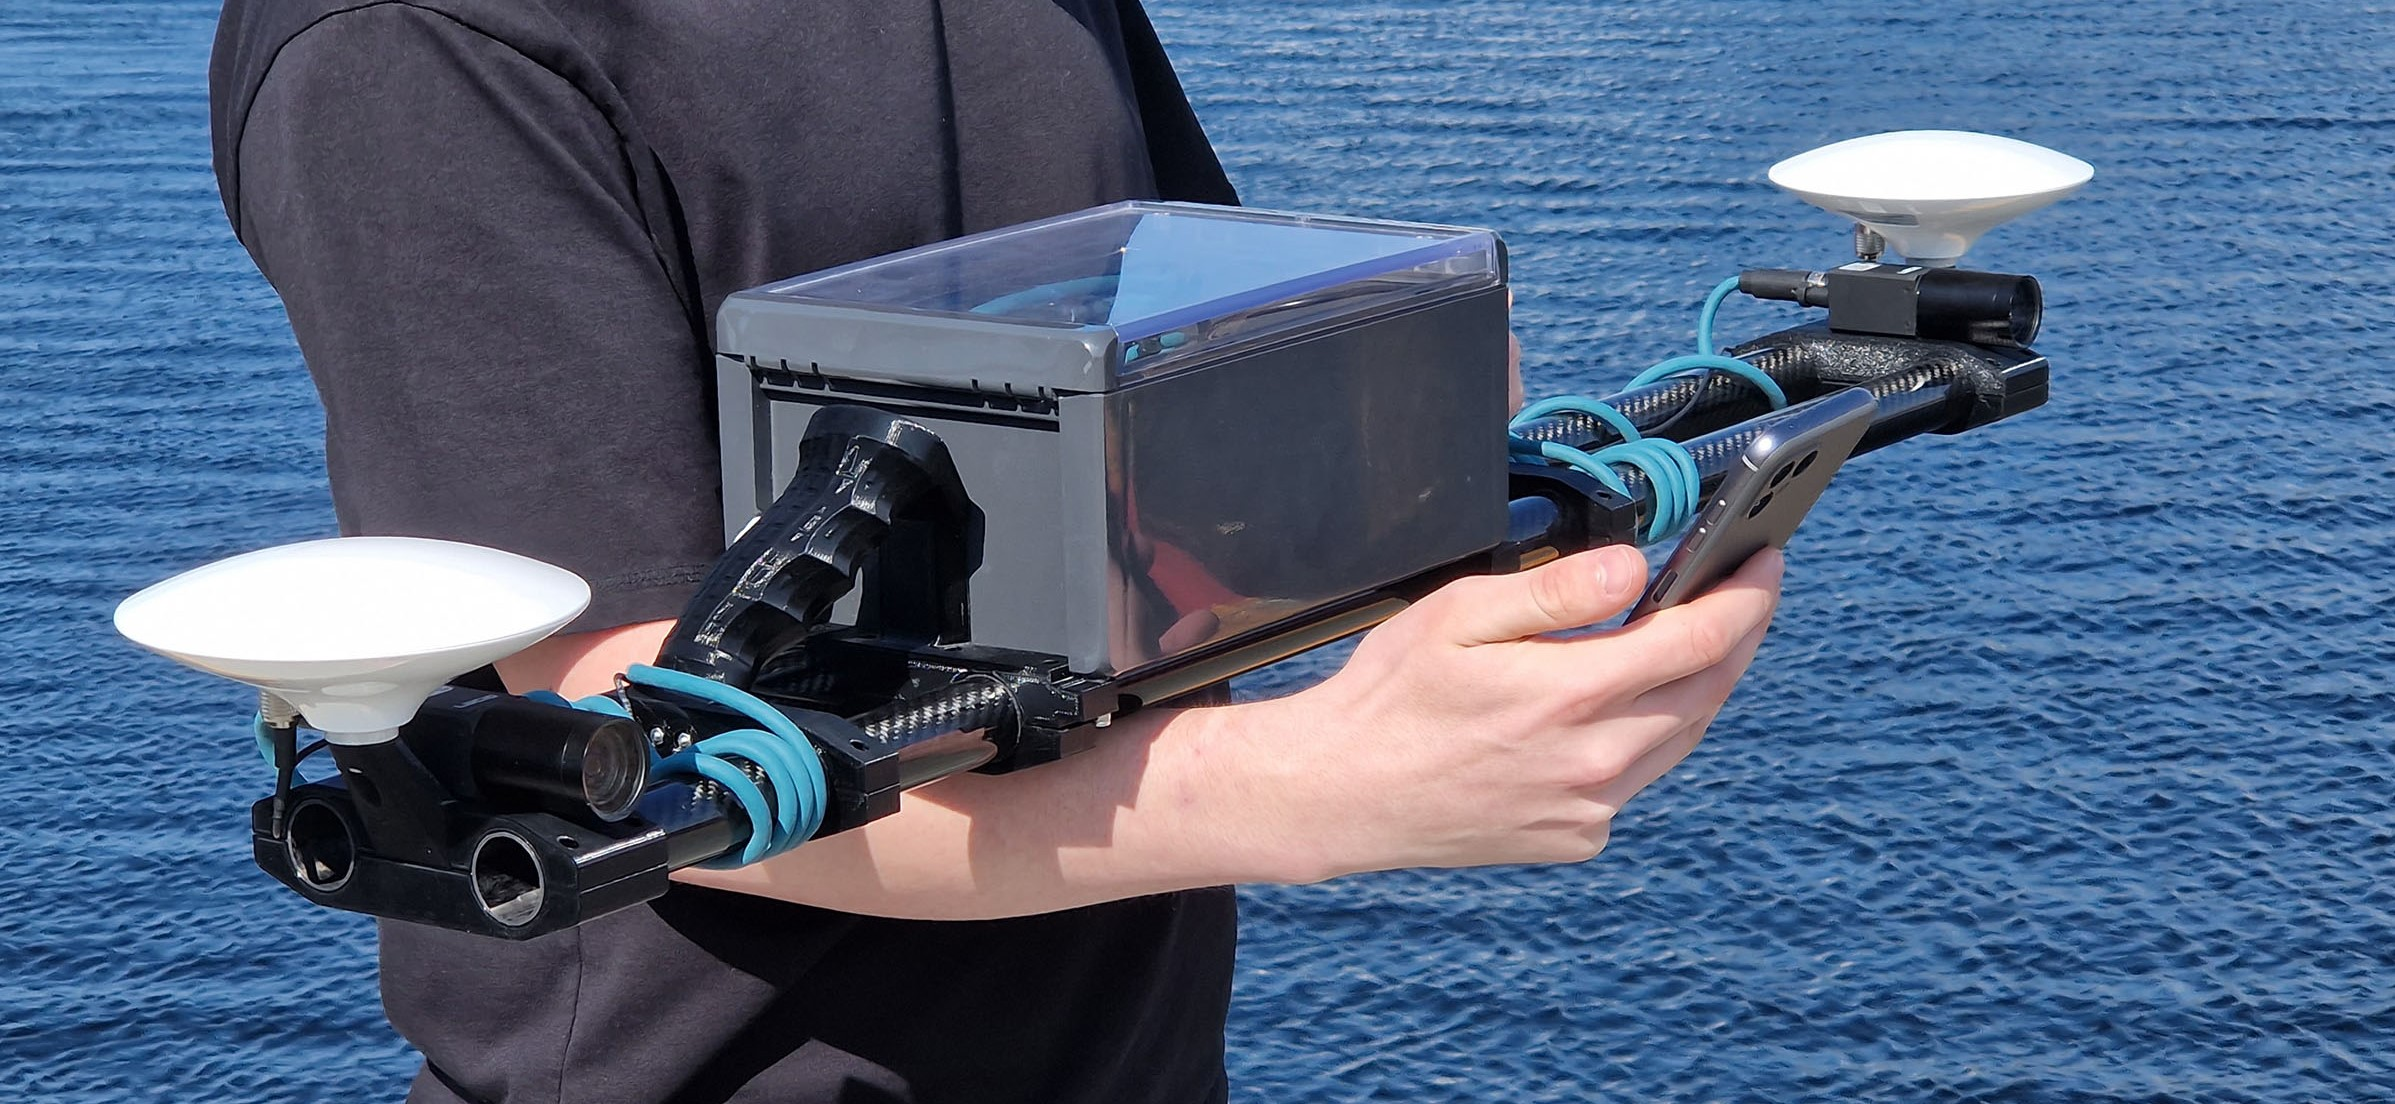
\includegraphics[width=\textwidth]{figures/operation.jpg}
    \caption{Operation of the sensor rig}
\end{figure}


\begin{figure}[H]
    % \centering
    \subcaptionbox{"Regular" image.}{
        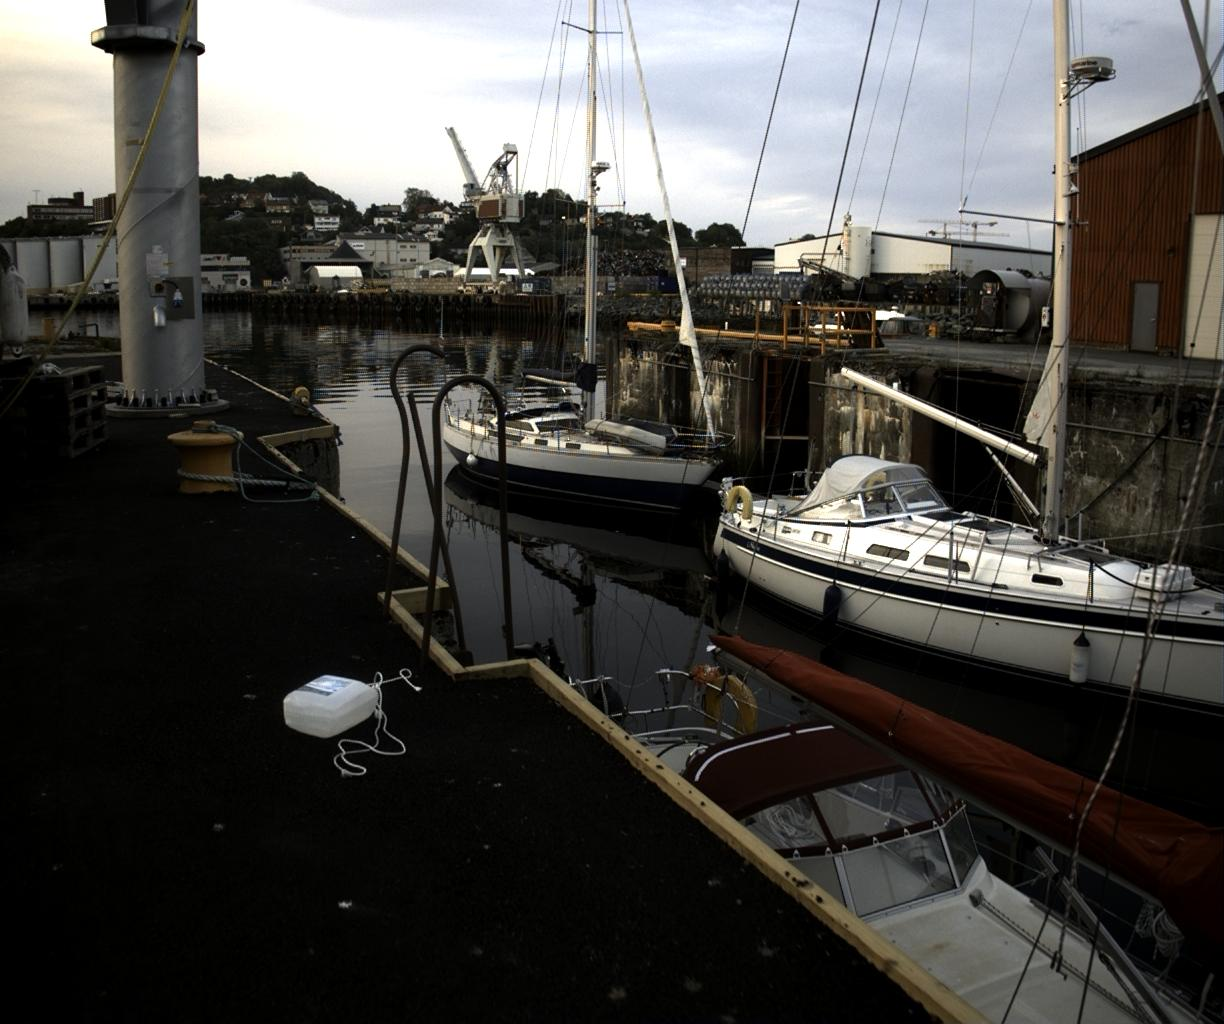
\includegraphics[width=0.48\textwidth]{figures/regular_right_96.jpeg}
    }
    \hfill
    \subcaptionbox{\glsentrylong{aolp} and \glsentrylong{dolp} visualized as hue and value.}{
        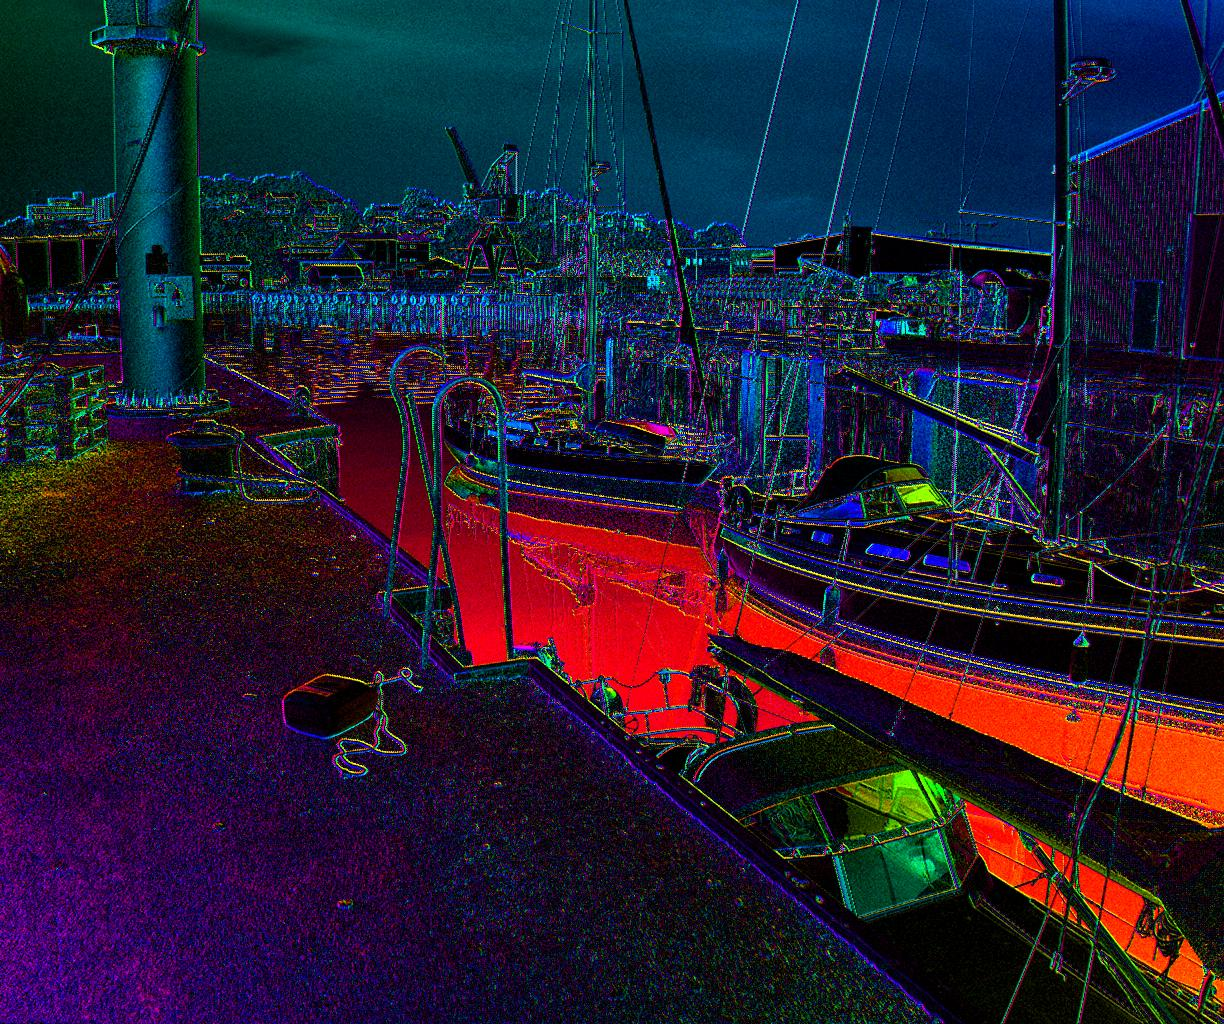
\includegraphics[width=0.48\textwidth]{figures/aolp_right_96.jpeg}
    }
    \caption{Illustration of how polarization cameras make the water surface visible.}
    \label{fig:polarization_visualization}
\end{figure}


\end{document}